\documentclass[runningheads]{llncs}

\usepackage{graphicx}
% Used for displaying a sample figure. If possible, figure files should
% be included in EPS format.
\usepackage{float}

\begin{document}
	%
	\title{Simulation Paper}
	
	\author{Benjamin Vandersmissen\inst{1} \and
		Lars Van Roy\inst{2} \and \\
		Evelien Daems\inst{3} \and
		Frank Jan Fekkes\inst{4}}
	%
	\authorrunning{B. Vandersmissen, L. Van Roy, E. Daems, F.J. Fekkes}
	% First names are abbreviated in the running head.
	% If there are more than two authors, 'et al.' is used.
	%
	\institute{
		\email{benjamin.vandersmissen@student.uantwerpen.be} \and
		\email{lars.vanroy@student.uantwerpen.be} \and
		\email{evelien.daems@student.uantwerpen.be} \and
		\email{franciscus.fekkes@student.uantwerpen.be}}
	%
	\maketitle              % typeset the header of the contribution
	%
	\begin{abstract}
		As described within the following paper, we have analyzed the extend of the randomness factor within Stride, the extinction threshold (aka the point at which no outbreaks occur), we have estimated factors like the immunity level and r0 for a given result, we have analyzed the individual influence of factors like demography, vaccines, commuting to work and finally we have performed a couple of benchmarks to see which aspects of the code where the most demanding. All of these analyses (wherever needed of course) are based upon an average of multiple seeded runs, and all results are obtained by analyses over a range of values, rather than a predetermined range/goal. We have for example been able to prove that commuting to work, contrary to expectations, on its own, does not affect the spreading of diseases in a significant manner. We have also been able to prove that vaccines, on their own, do affect the spreading of diseases. In general, we have found out that the individual parameters have little to no significant effect on their own, but that it is always a combination of parameters that influences the spread of a disease.

		
		%\keywords{First keyword  \and Second keyword \and Another keyword.}
		
	\end{abstract}
	
	
	\section{Introduction}
	In this paper we will discuss a couple of the aspects that are part of stride, as well as a brief look towards a couple of possible factors that may or may not influence the spreading of diseases (this will be proven by the analyses). Every aspect will be analyzed individually, so we will not do any analysis on correlations of parameters. All analyses regarding these factors will be done by performing multiple seeded runs where the average will be considered our final result. Finally, we will do a couple of benchmark runs where we vary some of the parameters, in order to determine which types of parameters affect the runtime of Stride, as well as an attempt on determining why this is the case. \\
	\\
	The paper itself will consist out of a simulation section, where we will perform a regular simple simulation, as well as an analysis on a couple of parameters, and their expected value, regarding a given simulation result. After the simulation section we have a section regarding the generation of populations. This section will quickly analyze the effect of a couple of parameters, on their own. The paper will end with the benchmark section where we will quickly demonstrate and explain our findings about the performance of different sections of code.
	
	\section{Simulation}
	
	\subsection{Introduction}
	The following subsections will contain a first view of the Stride tool along with a description of its output, as well as an estimation for the extinction threshold and a few simple analyses in order to approach used values for a given evolution of a disease within a population.
	
	\subsection{Stochastic variation}
	We use the Stan (STochatsic ANalysis) controller to examine the impact of stochasticity on the results obtained from the simulation. For this analysis we used a total of 15 simulations, since these will suffice to show the effects of randomness within the stride tool. More simulations and the resulting graph would no longer be clear, less simulations and the resulting graph might not properly display the differences.\\ 
	\\
	In Figure \ref{stochastic_analysis.png} the number of cumulative cases (total amount of infected persons) per time-step is plotted. Here we can observe an exponential growth of the number of cases throughout time. This is not surprising because it can be deducted from common reasoning. If per iteration more people are affected, a larger contactpool is possibly infected, the newly diseased will enter their personal contactpool and again more people will be reached.\\ 
	\\
	Towards the end a flattening of the curve occurs. This is not something totally unexpected because the population is obviously not infinite. At one point anyone who can be infected will effectively become a carrier of the disease. Something else that is important to note, are the flat lines at the bottom of the graph. These are what we call extinctions and they represent the evolution of diseases that died out.\\ 
	\\
	In order for these simulations to stand out more, a different number of seeding rate(the percentage of the population that starts out as being diseased). This allowed for a quicker climb in a shorter amount of time. Starting out with a lower number might/could have given us the same results (it definitively could, but its not given that it would due to the randomness) but it would take longer to show real differences, as they would all start out the same way.\\
	\\
	We can clearly see that randomness plays a major role within Stride, considering that there are two big sets of curves, the ones following an upward curve and the ones that go extinct, we cannot base conclusions on a small set of simulations as these might all be very different, we will from now on consider large sets of runs to determine the true expected evolution of a disease.\\
	
	\begin{figure}
		\centering
		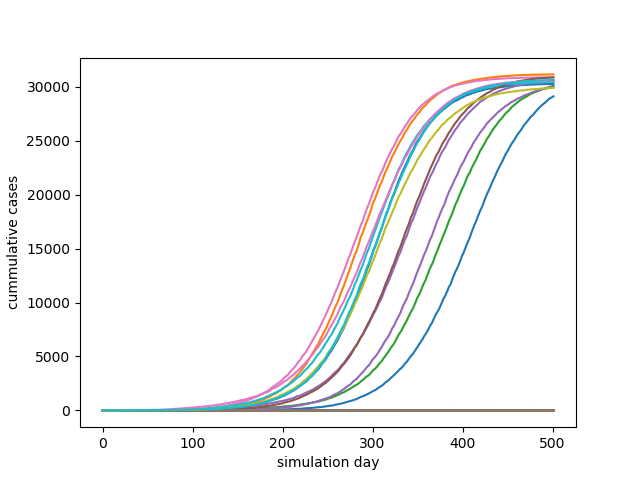
\includegraphics[width=0.90\textwidth]{stochastic_analysis.png}
		\caption{Result of 15 stochastic runs. The figure displays the distribution of the number of cummulative cases per time-step.} 	
		\label{stochastic_analysis.png}
	\end{figure} 
	
	
	\subsection{Determining an extinction threshold}
	Looking at figure \ref{stochastic_analysis.png} it is clear that in some cases an outbreak doesn't occur. These cases can be called extinctions of the outbreak or disease. Determining if a simulation is an extinction or an outbreak is neccessary to be able to divide the two possible outcomes. If we can find some threshold where there is a clear difference between large outbreaks and extinctions we can seperate the two scenarios.\\ \\
	After running fifty simulations we can plot the total number of infected cases and their frequency.  We used the file "stochastic\_analysis.xml" for the simulations. After running the simulator the outcome is plotted in the histogram in Figure \ref{fig3} where the frequency of the amount of infected cases is plotted.\\ \\
	There is a clear distinction between large outbreaks and smaller ones. The smaller ones are again plotted in the second histogram "extinction\_small.jpg". There it can be noticed that small outbreaks are really small (20 maximum). Which can be called an extinction afterIt is neccessary to be able to exclusively look at outbreaks.  500 days. The threshold for this example can be set between than 50 and 25 000. Either of those thresholds should eliminate all extinctions in this case.\\ \\
	A very low threshold might allow some extinctions to be passed while a high threshold might eliminate an outbreak. What can be noticed is the total lack of simulations between 100 and 25000 infected cases. But there can still be exceptions in the infected cases. A threshold of 1000 would be more than adequate. It will eliminate all extinctions while keeping the outbreaks.\\ \\
	It should be noted that this threshold will change for a lot of variables. For example: time and population will affect the threshold. A new threshold should be determined for each set of simulations.
	
	\begin{figure}
		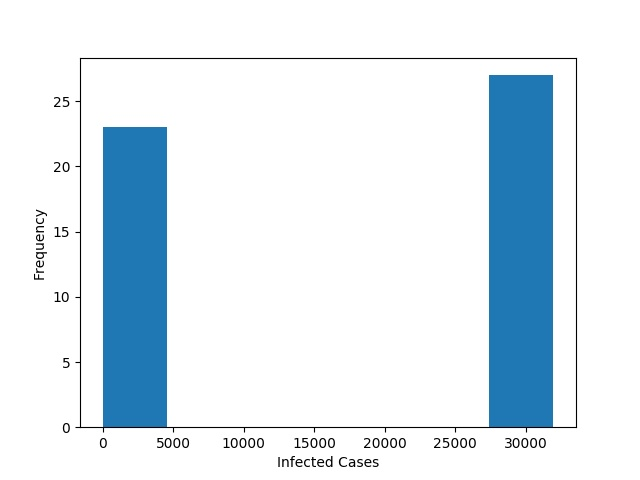
\includegraphics[width=\textwidth]{extinction_all.jpg}	
		\caption{Above is an histogram with the frequency of total infected cases for 50 simulations. See fig \ref{fig4} for an enlargement of the left spike.}
		\label{fig3}
		
		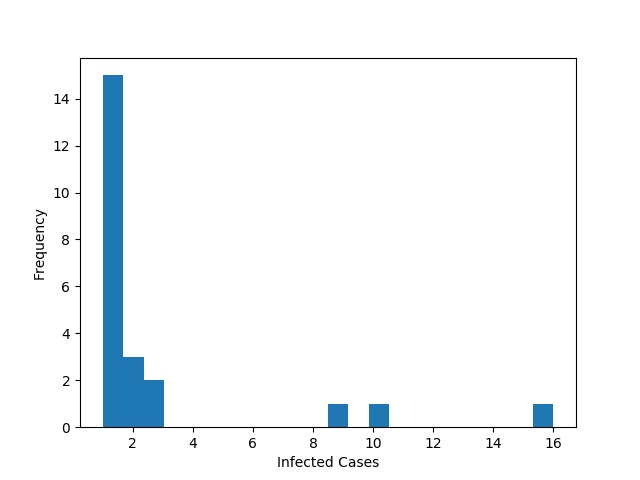
\includegraphics[width=\textwidth]{extinction_small.jpg}
		\caption{A zoom on the left spike of figure \ref{fig3}. Instead of 0 to 5000 it is actually 0 to 16.}	
		\label{fig4}
	\end{figure}
	\newpage
	
	\subsection{Estimating the immunity level}
	For this assignment we had to estimate the percentage of people who were immune to the disease given the following graph.
	\\ 
	\begin{figure}[h!]
		\includegraphics[width=\textwidth]{original.png}
		\caption{New cases observed per day during the outbreak}
	\end{figure}
	\newpage
	As a first approximation we performed 25 simulations for each immunity level with immunity levels ranging from 0 to 90\% as seen in figure \ref{fig5}. As we can clearly see, all immunity levels lower than 50\% are unrealistic for this scenario. As a next step we decided to drop off these immunity levels and generated a zoom of the realistic immunity levels with the same offset.
	\begin{figure}
		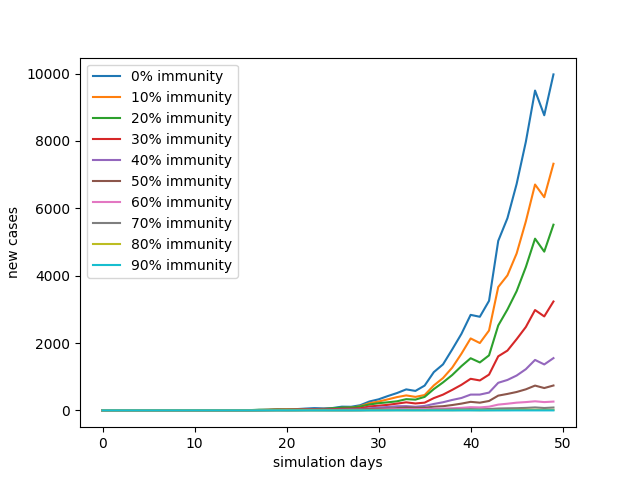
\includegraphics[width=\textwidth]{test_immunity_0-100.png}
		\caption{first estimate of outbreaks}
		\label{fig5}
	\end{figure}
	\newpage
	
	\newpage
	\noindent
	By dropping all percentages lower than 60 and higher than 80\% we get the following graph, this graph is a lot closer to the desired graph (since the highest number of new cases is now only 90 compared to over 10000), but is still far from accurate. We can now see that the desired immunity rate should lie somewhere between 70 and 80\%.	
	\begin{figure}
		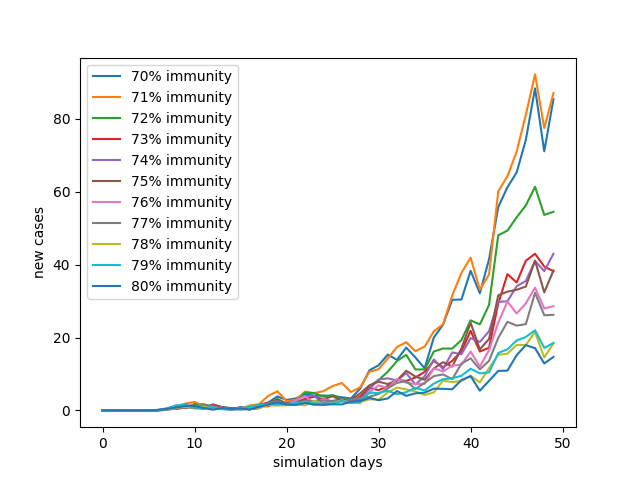
\includegraphics[width=\textwidth]{test_immunity_70-80.png}
		\caption{narrowed down estimate of outbreaks based on 25 simulations}
	\end{figure}
	
	\newpage
	\noindent
	Finally, we zoom in between 70 and 75\% and we can see that the immunity percentage is somewhere around the 70\% mark. Curiously enough, with an immunity rate of 71\% and an average of 25 simulations, there are more infected than with an immunity rate of 70\%. The only problem with this 70 \% graph is that there is a sudden drop in infections around day 45 while the original graph doesn't feature that drop.
	\begin{figure}
		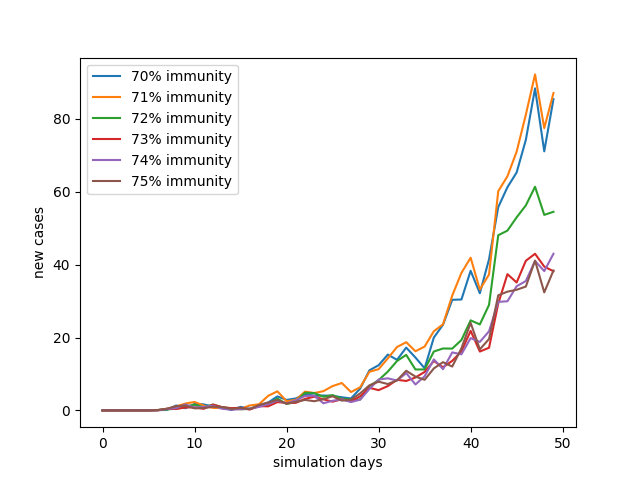
\includegraphics[width=\textwidth]{test_immunity_70-75.png}
		\caption{final estimate of outbreaks based on an average of 25 simulations}
	\end{figure}
	\newpage
	
	\subsection{Estimating R\textsubscript{0}}
	Here, we need to approximate the same graph but now he have to use an extra parameter, R\textsubscript{0}, the basic reproduction number of a disease, indicating how many people a single infected person will infect.
	\\
	\\
	\noindent
	We will use the same technique we used in the previous assignment, only this time, we need to repeat it for R0 = 12 .. 18.
	
	\begin{table}
		\begin{center}
			
			\begin{tabular}{c||c}
				R0 & estimated immunity rate \\ \hline
				12 & 65	\% \\
				13 & 68 \\
				14 & 69 \\
				15 & 70 \\
				16 & 73 \\
				17 & 74 \\
				18 & 76 \\
			\end{tabular}
			\caption{Estimated Immunity Rates based on 25 simulations}
		\end{center}
		
	\end{table}
	
	Generally speaking, there is an correlation between the immunity rate and the parameter R0.
	
	\begin{figure}
		\includegraphics[width=\textwidth]{test_R0_final.png}
		\caption{25 simulations for found immunity values} 
	\end{figure}
	
	\newpage
	\noindent
	\section{Population generation}
	
	\subsection{Investigating the influence of demography on epidemics}
	We generate populations for two regions with different age distributions. We need to find which region is more likely to have an outbreak, region A, which has more younger people or region B, which has more elderly people.	
	\\
	\\	
	\noindent
	First we need to calculate the extinction thresholds for population A and population B. We do this in the same way as we did in 2.3. For population A, after 50 runs, we either have less than 10 cases or around 98.000 cases. We determine 1000 as the outbreak threshold, to leave some room for randomness. For population B, after 50 runs, we either have less than 10 cases or around 94.000 cases. We determine 1000 as the outbreak threshold for population B as well.
	\\
	\\
	\noindent
	In case of population A there is around an 80\% chance for an outbreak to occur, in the simulations with population B there is 73\% chance for an outbreak. Population B is the older population in respect to population A, this means that an older population does not mean an increase in the likelihood of an outbreak, but a decrease. A reasonable explanation for this could be the fact that in population B there are more working people than in population A. The average working person has a better immune system than a child and also has smaller contact matrices. Population B also has more retired people than population A and those retired people have an even smaller contact pool.
	
	\begin{figure}
		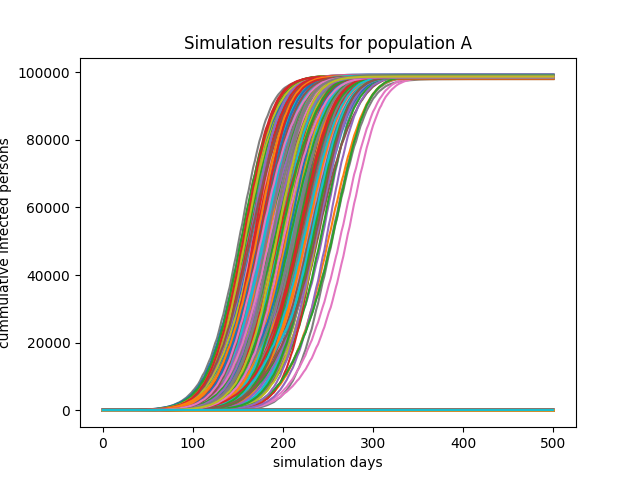
\includegraphics[width=\textwidth]{outbreaks_populationA.png}
		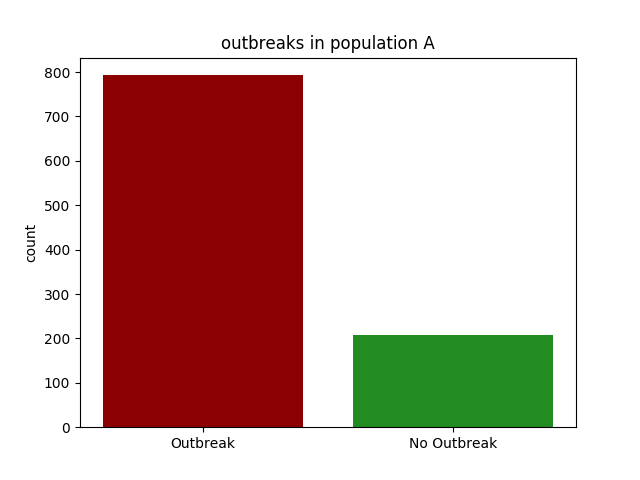
\includegraphics[width=\textwidth]{barchart_populationA.png}
		\caption{Results of 1000 simulations with population A}
	\end{figure}
	\begin{figure}
		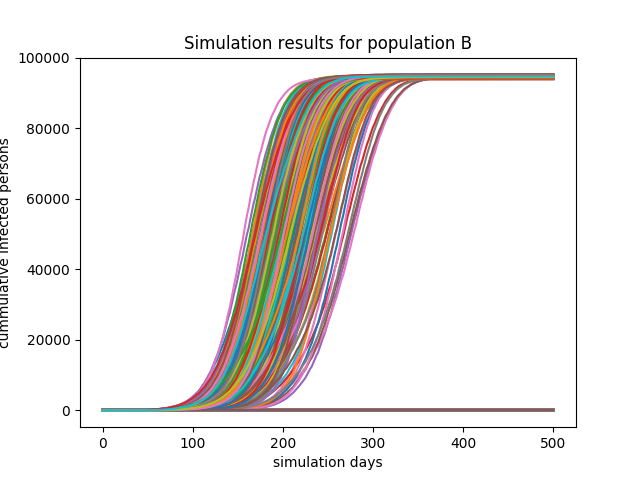
\includegraphics[width=\textwidth]{outbreaks_populationB.png}
		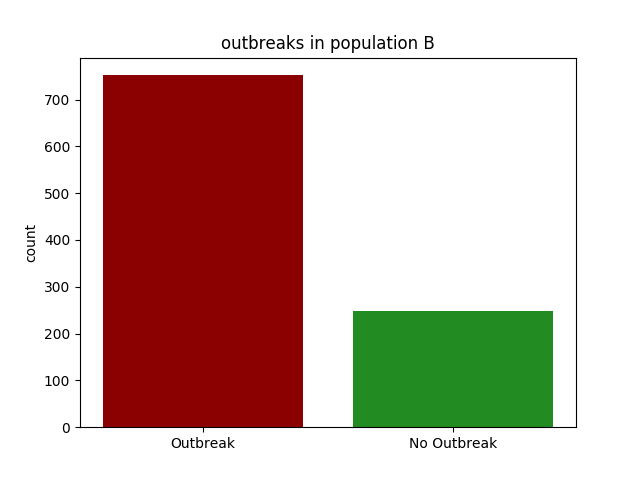
\includegraphics[width=\textwidth]{barchart_populationB.png}
		\caption{Results of 1000 simulations with population B}
	\end{figure}
	\newpage
	\noindent
	\subsection{Vaccinating on campus}
	%redo the image => confine vaccination to student and not to age group
	Vaccinations are often given at a young age. But not everyone gets vaccinated, there might be particular groups of people who are more susceptible. Here it is simulated what would happen if student were such a group. A student will be defined as a person between the age of 18 and 26 who are in the pool "College". A population will be generated where the age group of 18 to 26 will have  a lower immunity. To test if vaccinating the students during an outbreak will aid in the surpression of it, two scenario's will be tested. One where the students will be vaccinated a week after an infected individual is introduced and one where the students aren't vaccinated.\\
	A total of 100 simulations have been run. 50 Without vaccinations and 50 with vaccinations given seven days after the first infected individuals are introduced. A total of 1200 people will be infected to start the outbreak. The cumulative infected cases have been tracked from day to day and averaged over all simulations. The results are shown on fig \ref{vax_campus}. The results are averaged because there wasn't much deviation between the runs but a single run isn't a good representation.\\ \\
	It is clear that even vaccinating during an outbreak helps in surpressing said outbreak. With only around 3500 students needing a vaccination in a studentbody of around 60000 and a total population of ten times that, the cost saving is quite hight and the amount of infected is reduced. \\
	In conclusion, vaccinating students who still need their vaccinations, is worth it during an outbreak in this scenario.
	
	\begin{figure}[h!]
		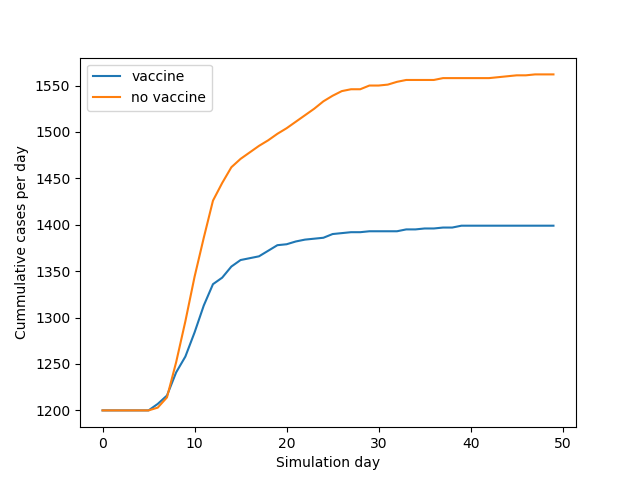
\includegraphics[width=\textwidth]{student_vaccinations.png}
		\caption{Above is a plot of average cumulative cases of 50 simulation each seen day by day. People between the age of 18 and 26 have a lowered immunity against the disease. During the blue scenario people in college are vaccinated after seven days. They are not in the orange scenario.}
		\label{vax_campus}
	\end{figure}
	\clearpage
	
	\subsection{Is commuting to work important for disease spread?}
	One could easily assume that working at a different location affects the rate at which a disease spreads, as it enhances it's reach. To get an idea of the effect of the parameter we did a simulation for 6 different percentages, ranging from 0 to 100. The displayed data are an average derived from 30 different runs for each percentage. In order to obtain these results, "general" values for all other parameters were used so that we would only look at the effects of commuting, rather than the combined influences of multiple parameters. \\
	\\
	\noindent 
	It is true that taking an average might devalue part of the estimation of the data, therefore we made a boxplot of the found data, to see what the biggest outliers were, and how far the mean was from the average run. We can clearly see that there are little to no outliers and that all the data is more or less centralized around the actual found average.
	\begin{figure}
		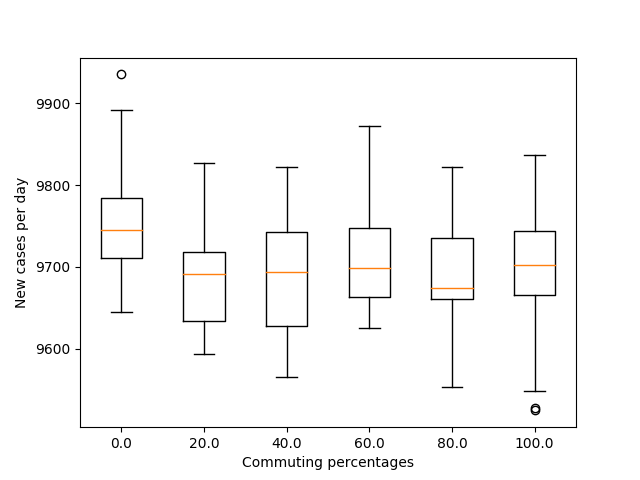
\includegraphics[width=\textwidth]{commuting_boxplot.png}
		\caption{Boxplot made from final infection counts derived from 30 runs per percentage.}
	\end{figure}
	
	\noindent
	Now for the actual graph, we can't see any obvious difference between the different runs, on this scale. The same can be seen from the boxplot, where the general result is all within a very similar range. There are differences, but these could just be related to the randomness of stride, and they do not have to be specifically caused due to the commuters. 
	
	\begin{figure}
		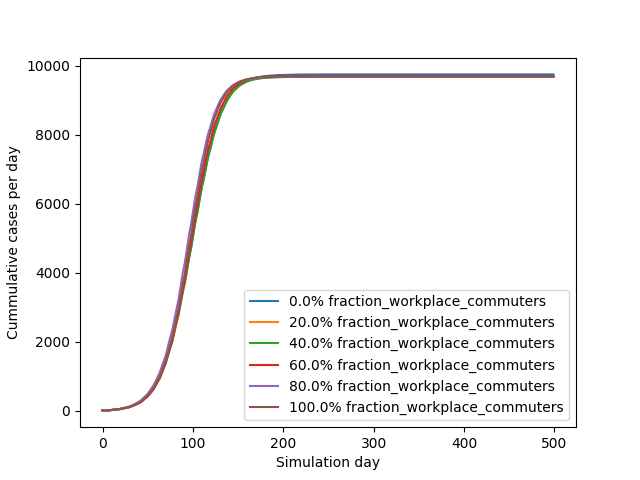
\includegraphics[width=\textwidth]{commuting_cumul.png}
		\caption{Results of 6 different percentages of commuters in a range from 0 to 100.}
	\end{figure}

	\noindent
	As a conclusion I would say that there might be small effects of the percentage of commuters, as the results are not identical, however the differences are so small that these might as well be due to randomness. I do not think that the percentage on its own will be significant to the final results.
	
	\newpage
	\section{Performance profiling of sequential code}
To study the performance of the code we will discuss a few parameters. We used the GPROF tool to profile the code. Based on these result we could see the influence of different parameters on the runtime.

\subsection{Number of days}
A simulation is ran for a random number of days (this randomness is not based on a random generator but we increasingly altered the number of days and showed the meaningful results in this paper) and then we look at the time needed to complete the algorithm. \\ 
\\
As could be expected, there is an increase in execution time when we take a larger amount of days. The number of days determines the number of loops in a simulation, hence this logically affects the needed time for a simulation by quite a big margin. We have noticed that throughout this performance analysis, this parameter is one of the largest causes of a big difference in performance. Especially the sorting of the members and getting the total amount of infected people took up most of the computing time.\\
From the graph in Figure 14 a linear relation can be noticed between the number of days for which a simulation is ran and the time the simulation needed to end completely. If we would continue to enlarge the number of days this linear growth will continue.

\begin{table}
	\caption{Relation between the number of days and the runtime}
	\begin{center}
		\begin{tabular}{ | c | c |}
			\hline
			Number of days & Time needed for SimRunner and SimController to end \\ \hline
			10 & 00:00:01:675:260 \\ \hline
			50 & 00:00:03:427:244 \\ \hline
			100 & 00:00:06:088:121 \\ \hline
			500 & 00:00:17:981:791 \\ \hline
			1000 & 00:00:33:047:163 \\ \hline
			2000 & 00:01:02:011:203 \\
			\hline	
		\end{tabular}
	\end{center}
\end{table}
\newpage
\begin{figure}
	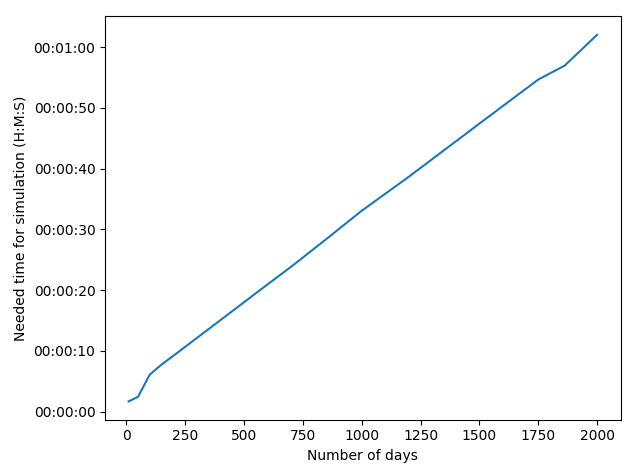
\includegraphics[scale=0.65]{performance_days.png}
	\caption{Relation between the number of days and the time needed to complete a simulation.} 
\end{figure}

\subsection{Population size}
Next, we vary the parameter of population size. From the data in Table 3 it is clear that the larger the population the longer the simulation needs to finish (this simulation includes generating the population). This is also ,oticable in Figure 15 were the simulation runtime grows rapidly with an increasing population size. If an existing population is used we have noticed that a simulation takes less time to complete which is what could be expected. From the GPROF analysis we notice that the most work is done in getting the count of the infected and sorting the members. \\

It can be said that the size of the population delivers the most influence on the total time. One can argue that the number of days had the most impact but it is not completely realistic to study outbreaks over a number of years what would take up the most computation time. But this argument is overthrown since an outbreak of a disease can be modeled for quite a long time (for centuries) and thus is the size of the population as important as the duration of a simulation.\\

In the previous part we considered the impact of the number of days and concluded this is a large factor in the time needed to complete a study of an outbreak. And as could be expected a large number of days combined with a large population will result in a large execution time.

\begin{table}
	\caption{Relation between population size and simulation runtime (including generating population)}
	\begin{center}
		\begin{tabular}{ | c | c |}
			\hline
			Population size & Time needed \\ \hline
			1000 & 00:00:00:429:476 \\ \hline
			50000 & 00:00:00:620:702 \\ \hline
			100000 & 00:00:00:954:298 \\ \hline
			500000 & 00:00:03:904:541 \\ \hline
			1000000 & 00:00:07:272:251 \\
			\hline	
		\end{tabular}
	\end{center} 
\end{table}
\begin{figure}
	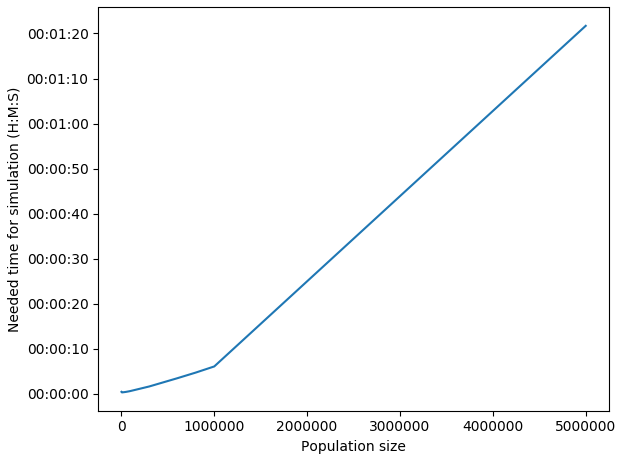
\includegraphics[scale=0.65]{performance_population.png}
	\caption{Relation between the size of the population and the time needed to complete the simulation} 
\end{figure}
\newpage

\subsection{Generating a population}
When considering the time needed to only generate a geo-based population and write it to a file without performing a simulation, the tendency of an increasing time with a larger population can be observed. The most computing power went to writing the contact pools for the population.

\begin{table}
	\caption{Relation between population size and generating runtime}
	\begin{center}
		\begin{tabular}{ | c | c |}
			\hline
			Population size & Time needed \\ \hline
			1000 & 00:00:00:262:863 \\ \hline
			10000 & 00:00:00:308:607 \\ \hline
			100000 & 00:00:00:336:115 \\ \hline
			500000 & 00:00:01:130:983 \\ \hline
			1000000 & 00:00:02:386:551 \\
			\hline
		\end{tabular}
	\end{center}
\end{table}

\subsection{Immunity rate}
When varying the immunity rate, there is no significant difference in runtime for different configurations. In order for this variable to have an influence on the final result, it is necessary to give other parameters different values.  As mentioned earlier, most of the time is used to sort and analyze the population, a factor like immunity rate has no effect on this process. In the table below you can see the runtimes for different immunity rates and a period of 50 days. When performing this analysis with a higher number of days of course this took some more time. But changing the immunity itself has no effect.

\begin{table}
	\caption{Relation between immunity rate and simulation runtime}
	\begin{center}
		\begin{tabular}{ | c | c |}
			\hline
			Immunity rate & Time needed \\ \hline
			0.2 & 00:00:04:869:367 \\ \hline
			0.4 & 00:00:04:873:811 \\ \hline
			0.6 & 00:00:04:966:409 \\ \hline
			0.8 & 00:00:05:035:361 \\ \hline
			0.99 & 00:00:04:921:399 \\
			\hline	
		\end{tabular}
	\end{center}
\end{table}

\newpage
\subsection{Seeding rate}
Seeding rate has a slight impact, but this impact is minimal. Seeding rate has no effect on the computation needed to sort and analyze the population, which is the major faction in a simulation. This minimal impact comes from initializing the population with the right amount of infected people or any other healt status. The following observations were made with a number of days equal to 50. A larger amount of days combined with the various different seeding rates had no significant larger performance weight than the times we could observe at the number of days section.

\begin{table}
	\caption{Relation between the seeding rate and the simulation runtime}
	\begin{center}
		\begin{tabular}{ | c | c |}
			\hline
			Seeding rate & Time needed \\ \hline
			0.000001 & 00:00:06:210:017 \\ \hline
			0.00001 & 00:00:06:188:449 \\ \hline
			0.0001 & 00:00:06:294:636 \\ \hline
			0.001 & 00:00:06:659:908 \\ \hline
			0.01 & 00:00:07:437:776 \\ \hline
			0.1 & 00:00:07:406:320 \\
			\hline	
		\end{tabular}
	\end{center} 
\end{table} 

\subsection{Contact log mode}
The contact log mode has a significant impact on the running time of a simulation. When the standard algorithm is used (all or susceptibles) it requires a lot more time to complete the simulation. This is because for every persons in a contactpool the algorithm will loop over all its possible contacts and makes no smart choices in the beginning opposed to the optimized algorithm. It forms a large contrast with the running time needed when using the optimized algorithm with all the members of the contact pool sorted. By reducing the number of loops in the algorithms, the necessary time to complete the algorithm can be reduced along with it.

\begin{table}
	\caption{Relation between the contact log mode and time needed to perform a simulation.}
	\begin{center}
		\begin{tabular}{ | c | c |}
			\hline
			Contact log mode & Time needed \\ \hline
			All & 00:18:38:106:723 \\ \hline
			Susceptibles & 00:18:20:352:080 \\ \hline
			None & 00:00:06:620:969 \\ \hline
			Transmissions & 00:00:06:793:748 \\
			\hline	
		\end{tabular}
	\end{center}
\end{table}
\end{document}

